\documentclass[10pt,a4paper]{article}
\usepackage[utf8]{inputenc}
\usepackage{ae}
\usepackage[brazil]{babel}
\usepackage[vmargin=2cm,hmargin=2cm,columnsep=0.75cm]{geometry}
\usepackage{float,nonfloat}
\usepackage{graphicx,color}
\usepackage{subcaption}
\usepackage{amsmath}

\makeatletter
\let\@institution\empty
\def\institution#1{\def\@institution{#1}}
\renewcommand{\maketitle}{
    \begin{center}
        {\Large\bfseries\@title\par\medskip}
        {\large
            \begin{tabular}[t]{c}%
                \@author
        \end{tabular}\par\medskip}
        {\itshape\@institution\par}
        {\itshape\@date\par}
\end{center}}
\makeatother

\newcommand{\pixel}{\textit{pixel} }
\newcommand{\pixels}{\textit{pixels} }

\begin{document}
% ============================================================================

\title{MC920: Introdução ao Processamento de Imagem Digital\\Tarefa 2}
\author{
    \begin{minipage}{6cm}
        \centering
        Martin Ichilevici de Oliveira\\
        RA 118077
    \end{minipage}
    \and
    \begin{minipage}{6cm}
        \centering
        Rafael Almeida Erthal Hermano\\
        RA 121286
    \end{minipage}
}
\institution{Instituto de Computação, Universidade Estadual de Campinas}
\date{\today}

\maketitle

% ============================================================================

O dominio do processamento espacial de imagem é aplicado ao plano da imagem, enquanto o dominio do processamento de frequencia da imagem é a modificação da transformada de Fourier da imagem.

O dominio espacial se refere aos pixels que compoem a imagem. Operações espaciais podem ser denotadas como sendo uma transformação:

\[g(x,y) = T[f(x,y)]\]

Em que $f(x,y)$ é a imagem original e $g(x,y)$ é a imagem processada.

$T[f(x,y)]$ pode ser aplicada em levando em conta uma vizinhança do ponto $(x,y)$.

\section{Operações pontuais}

Se a vizinhança possui tamanho 1x1, temos uma operação pontual. Neste caso $T$ se transforma em um função de transformação de nível de cinza.

Alguns exemplos de operações pontuais são:

\begin{enumerate}
    \item Image negative: consiste na inversão nos níveis de intensidade dos píxels de uma imagem.
        \[T[f(x,y)] = L - f(x,y)\]

        Onde L é a cor máxima na escala de cinza.

    \item Log transformation: consiste em aumentar uma pequena faixa de cores da imagem.
        \[T[f(x,y)] = c * \log(1 + f(x,y))\]

    \item Power law transformation: Tal qual a transformação log, uma lei de potência consegue mapear uma faixa estreita de cores em uma faixa maior. Power law transformation é muito utilizada em transformações gama para correção de dispositivos de aquisição, como captura de raios x.

        \[T[f(x,y)] = c \cdot f(x,y) ^e\]

    \item Contrast stretching: consiste em escurecer os pixels que possuem nível de cinza abaixo de M e clarear imagens com nível de cinza acima de M. O resultado final desta operação é uma imagem binária.
        \begin{align*}
            T[f(x,y)] &= 0 \text{ se } f(x,y) < M \\
                      &= 1 \text{ se } f(x,y) > M
        \end{align*}

    \item Gray level slicing: Consiste em aumentar determinados níveis de cinza para destacá-los

    \item Bit-plane slicing: consiste em separar em camadas os níveis de cinza, por exemplo, se a imagem é composta de pixels de 8 bits, poderiam ser criados 8 camadas, uma para cada bit.

\end{enumerate}

\section{Operações Globais}
Caso a vizinhança a ser considerada para o cálculo de $T(r)$ considere (quase) todos os \pixels da imagem, então a chamamos uma operação global. Seja $s$ uma função que produz um nível de intensidade para cada \pixel da imagem de entrada. Consideremos transformações do tipo

\[ s = T(r) \qquad 0 \le r \le L -1 \],

em que $r$ é um nível de intensidade, $L$ é a intensidade máxima da imagem e $T(r)$ é uma função estritamente monotonicamente crescente no intervalo $[0, L-1]$. 

Podemos entender a distribuição de níveis de cinza em uma imagem como resultado de uma função aleatória, a função densidade de probabilidade. Esta função apenas diz a probabilidade de, dado um \pixel qualquer, observarmos uma certa intensidade e é denotada por $p_r(r)$ ou $p_s(s)$.

Dada a relação entre $s$, $r$ e $T(r)$, e assumindo que $T(r)$ é diferenciável, então a densidade de probabilidade de $s$ pode ser obtida por
\begin{equation}
    p_s(s) = p_r(r)\left|\frac{dr}{ds}\right|
    \label{eq:fdp}
\end{equation}

Uma função de grande importância no processamento de imagens é a função de distribuição cumulativa (FDC), que pode ser expressa por

\begin{equation}
    s = T(r) = (L-1) \int_0^r p_r(w)dw
    \label{eq:fdc}
\end{equation}

Podemos então calcular $p_s(s)$ para esta função, subsituindo a expressão \ref{eq:fdc} na expressão \ref{eq:fdp}.

\begin{align*}
    \frac{ds}{dr} = \frac{dT(r)}{dr} &= (L-1) \frac{d}{dr} \left[\int_0^r p_r(w)dw \right] = (L-1) p_r(r) \\
    \\
    p_s(s) &= p_r(r) \left|\frac{dr}{ds}\right| = p_r(r) \left|\frac{1}{(L-1)p_r(r)}\right|\\
           &= \frac{1}{L-1} \qquad 0 \le s \le L-1
\end{align*}

A formulação anterior assume que as funções são contínuas. Contudo, ao trabalhar com imagens digitais, trabalhamos com valores discretos. Em particular, a função de distribuição de probabilidade pode ser expressa por um histograma, cuja distribuição de probabilidade pode ser expressa pela Eq. \ref{eq:prob}.

\begin{equation}
    p_r(r_k) = \frac{n_k}{MN}
    \label{eq:prob}
\end{equation}

em que $n_k$ é a quantidade de \pixels com intensidade $r_k$ na imagem e $M$, $N$ são as dimensões da imagem. Substituindo \ref{eq:prob} em \ref{eq:fdc}, e substituindo a integral por um somatório (já que estamos lidando com uma função discreta), obtemos a expressão \ref{eq:hist_eq}.

\begin{equation}
    s_k = T(r_k) = \frac{L-1}{MN}\sum_{j=0}^k n_j
    \label{eq:hist_eq}
\end{equation}

A esta transformação denominamos equalização histogrâmica. Ela tem a característica de aprimorar o contraste de uma imagem, clareando \pixels claros e escurecendo \pixels escuros.

Aplicou-se o processo de equalização histogrâmica à Figura \ref{fig:original}, a qual foi convertida para uma imagem em tons de cinza, como mostra a Figura \ref{fig:src}. O resultado está na Figura \ref{fig:dst}. Os histogramas correspondentes estão nas Figuras \ref{fig:hist_src} e \ref{fig:hist_dst}. Como se pode observar pelos histogramas, o intervalo das intensidades foi expandido, com mais \pixels claros e \pixels escuros do que anteriormente. O resultado visual é claro - é possível, por exemplo, observar detalhes que estavam poucos claros na imagem original.

\begin{figure}[!ht]
    \centering
    \begin{subfigure}[ht]{0.45\textwidth}
        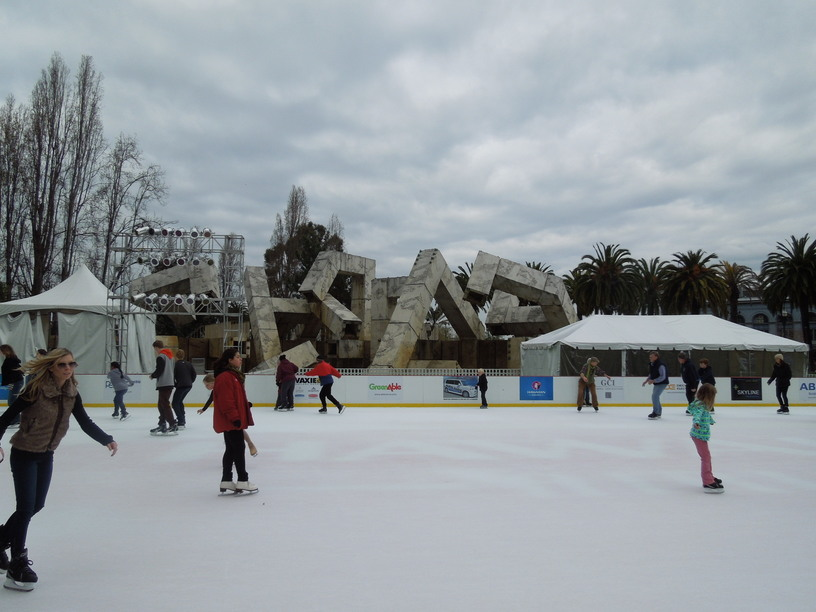
\includegraphics[width=\textwidth]{original.jpg}
        \caption{Figura original}
        \label{fig:original}
    \end{subfigure}
    \\
    \begin{subfigure}[ht]{0.45\textwidth}
        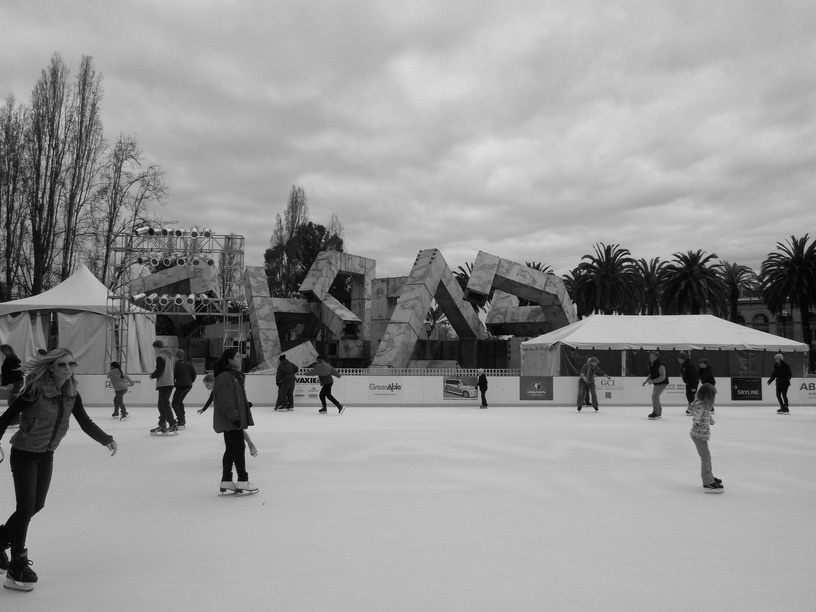
\includegraphics[width=\textwidth]{src.jpg}
        \caption{Antes da equalização histogrâmica}
        \label{fig:src}
    \end{subfigure}
    \qquad
    \begin{subfigure}[ht]{0.45\textwidth}
        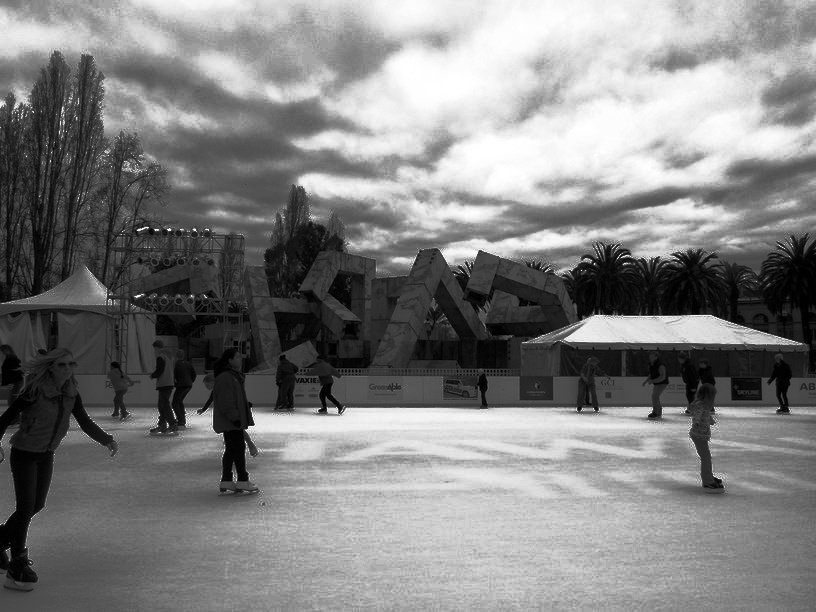
\includegraphics[width=\textwidth]{dst.jpg}
        \caption{Após equalização histogrâmica}
        \label{fig:dst}
    \end{subfigure}
    \caption{Imagem original e em tons de cinza antes e após equalização histogrâmica}
\end{figure}

\begin{figure}[!ht]
    \centering
    \begin{subfigure}[ht]{0.4\textwidth}
        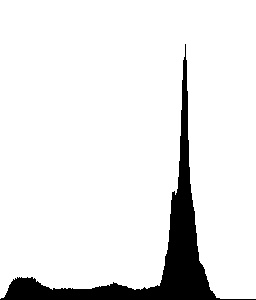
\includegraphics[width=\textwidth,height=\textwidth]{hist_src.jpg}
        \caption{Antes da equalização histogrâmica}
        \label{fig:hist_src}
    \end{subfigure}
    \qquad
    \begin{subfigure}[ht]{0.4\textwidth}
        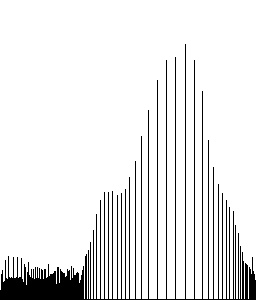
\includegraphics[width=\textwidth,height=\textwidth]{hist_dst.jpg}
        \caption{Após equalização histogrâmica}
        \label{fig:hist_dst}
    \end{subfigure}
    \caption{Histograma das Figuras \ref{fig:src} e \ref{fig:dst}}.
\end{figure}

\section{Operações de Vizinhança}
Algumas operações utilizam pequenas vizinhanças ao redor da imagem, essas operações são denominadas operações de vizinhança

Operações de vizinhança utilizam uma mascara ao redor do ponto $f(x,y)$.

Filtros lineares são o somatório do produto do coeficiente do filtro com o valor do pixel no ponto.

Alguns exemplos de operações de vizinhança:

\begin{enumerate}
\item Smoothing Linear Filters: consiste em substituir um pixel pela média dos pixels de sua vizinhança, para reduzir ruidos aleatórios.

\item Mediam filter: consiste em substituir o pixel pelo mediana dos pixels da vizinhança
\end{enumerate}


\begin{thebibliography}{99}
    \bibitem{livro} GONZALEZ, Rafael C.; WOODS, Richard E.. \textbf{Digital Image Processing}. 3. ed. Upper Saddle River, NJ, EUA: Prentice-hall, 2006.
    \bibitem{opencv} \texttt{http://docs.opencv.org/doc/tutorials/imgproc/histograms/histogram\_equalization/\\histogram\_equalization.html}
\end{thebibliography}

\end{document}
